\section{Обзор существующих библиотек}

В рамках исследования был проведен анализ существующих pretty printer библиотек на основе комбинаторов.
% возможно, рассказать о комбинаторах

\subsection{Библиотека Джона Хьюза}

Библиотека Джона Хьюза, описанная в \cite{hughes}, явялется первой комбинаторной pretty printing библиотекой. Она основана на алгоритме, предложенном Дереком Оппеном в \cite{oppen}, по сути является его реализацией в функциональном стиле на Haskell. Также библиотека Джона Хьюза, расширенная Саймоном Пейтоном Джонсом \cite{peytonJones}, является стандартной pretty print библиотекой для Haskell.

% рассказать об оптимальном

В данной библиотеке ключевым типом является \textbf{Doc}. Основные комбинаторы для составления документа:
\inputminted{haskell}{codes/hughesBasicOperators.hs}

Так с помощью функции \textbf{text} по строке получается документ, оператор \textbf{(<>)} соединяет два документа горизонтально (см. рисунок~\ref{fig:hughesHorComp}), а оператор \textbf{(\$\$)} соединяет документы вертикально (см. рисунок~\ref{fig:hughesVertComp}).

\begin{figure}[h!]
	\begin{minipage}[b]{0.45\linewidth}
		\centering
		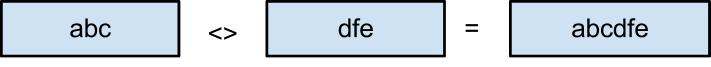
\includegraphics[width=\textwidth]{hughesHorComp}
		\caption{}
		\label{fig:hughesHorComp}
	\end{minipage}
	\hspace{0.5cm}
	\begin{minipage}[b]{0.45\linewidth}
		\centering
		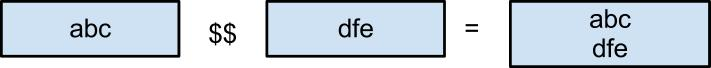
\includegraphics[width=\textwidth]{hughesVertComp}
		\caption{}
		\label{fig:hughesVertComp}
	\end{minipage}
\end{figure}

Элемент типа \textbf{Doc} может быть переведен в строку с помощью функции \textbf{pretty}.
\inputminted{haskell}{codes/hughesPretty.hs}
Кроме самого документа, функция \textbf{pretty} также принимает два числа: максимальную длину и максимальную наполненность строки. Здесь максимальная наполненность строки значит длину текста без выдущих пробельных символов.

